\providecommand{\main}{../../../..}
\documentclass[\main/dresen_thesis.tex]{subfiles}
\renewcommand{\thisPath}{\main/chapters/theoreticalBackground/scattering/introduction}
\begin{document}
  \subsection{Scattering Theory}\label{sec:theoreticalBackground:scattering:scatteringTheory}
    In general, scattering theory describes the scattering of particles, \textit{e.g.} neutrons or x-ray photons, from a scattering center as depicted in \reffig{fig:theoreticalBackground:scattering:scatteringTheory:scatteringProcess}. An incoming wave $\vec{k}_i$ with defined direction can interact with a scattering center and due to this deviate from its straight path, exiting as outgoing wave $\vec{k}_o$.
    If energy is conserved ($|\vec{k}_i| = |\vec{k}_o|$) the process is called elastic and otherwise inelastic.
    The vector describing the change from one momentum to the other is noted by
    \begin{align}
      \vec{q} \eq \vec{k}_o - \vec{k}_i.
    \end{align}
    For an elastic process the magnitude of $\vec{q}$ is directly determined by the wavelength $\lambda$ and angle $2\theta$ between $\vec{k}_i$ and $\vec{k}_o$ by
    \begin{align}
      |\vec{q}| \eq \frac{4 \pi}{\lambda} \sin(\theta),
    \end{align}
    where it is used that $|\vec{k}_i| \eq |\vec{k}_o| \eq k \eq \frac{2 \pi}{\lambda}$.

    \begin{figure}[tb]
      \centering
      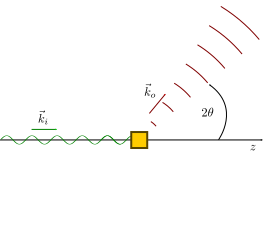
\includegraphics{scatteringTheory_scatterProcess}
      \caption{\label{fig:theoreticalBackground:scattering:scatteringTheory:scatteringProcess}General scattering process. An incoming wave with wave vector $\vec{k}_i$ (green) interacts with a scattering center (yellow) and produces an outgoing wave with wave vector $\vec{k}_o$ (red).}
    \end{figure}

    Scattering theory determines the transition probabilities for an particle to go from an incoming state to an outgoing state - respectively defined by their energy, momentum and polarization - in dependence of the properties of the particles, the scattering center and their interaction potential.
    Thereby it provides a method to calculate from a model the expected scattering intensity, which can be compared to an actual scattering experiment.
    In non-relativistic physics, \textit{e.g.} for neutrons, the problem that needs to be solved for this is the Schr\"odinger equation
    \begin{align}
      \label{eq:theoreticalBackground:scattering:scatteringTheory:schrodingerEquation}
      \bigg(\frac{\hat{p}^2}{2m} + V \bigg) \ket{\psi} \eq E \ket{\psi},
    \end{align}
    with the boundary condition $V(\vec{r}) \eq 0$ for $\vec{r}$ outside the scattering region.
    For electromagnetic waves such as x-rays, the propagation and interaction with matter is described best by quantum electrodynamics.
    For most cases, classical electrodynamics is however sufficient and in \refapp{ch:appendix:calculations:scatteringTheoryElectromagneticWaves} it is shown that the scattering theory from Maxwell's equations maps to the same type of problem as is discussed in the following for the Schr\"odinger equation.

    In scattering theory, it is assumed that the scattering particles are non-interacting among themselves, which is a well approximation for photons and neutrons.
    The interaction between the wave and the scattering center is described completely by $V(\vec{r})$ and is discussed in further detail in \refsec{sec:theoreticalBackground:scattering:interactionWithMatter}.
    To solve \refeq{eq:theoreticalBackground:scattering:scatteringTheory:schrodingerEquation}, the Hamiltonian is defined as
    \begin{align}
      H_0 &\eq \frac{\hat{p}^2}{2m},\\
      H &\eq H_0 + V,
    \end{align}
    and $\ket{\phi}$ is defined as the eigenstates of the free Schr\"odinger equation
    \begin{align}
      H_0 \ket{\phi} &\eq E \ket{\phi}.\\
    \end{align}
    Now, naively, the Schr\"odinger equation can be rearranged as
    \begin{align}
      \ket{\psi} &\eq \frac{1}{E - H_0} V \ket{\psi},
    \end{align}
    but this would not fulfil the boundary condition for $r \rightarrow \infty$, where $V\eq0$, and it has an ill-defined denominator for the eigenstates.
    Therefore, the correct solution needs the addition of the free particle solution and a definition how the pole is supposed to be treated.
    The latter is done by adding a infinitely small and positively complex value $i\epsilon$ to the denominator. The resulting equation
    \begin{align}
      \ket{\psi} &\eq \ket{\phi} +  \frac{1}{E - H_0 + i \epsilon} V \ket{\psi},
    \end{align}
    is known as the Lippmann-Schwinger equation and  it solves the Schr\"odinger equation by construction.
    In position space, it reads as integral equation
    \begin{align}
      \psi (\vec{r}) &\eq \phi(\vec{r}) + \int \dint \vec{r}^\prime \bra{\vec{r}}\frac{1}{E - H_0 + i \epsilon} \ket{\vec{r}^\prime} V (\vec{r}^\prime)\psi (\vec{r}^\prime),
      \label{eq:theoreticalBackground:scattering:scatteringTheory:LippmanSchwingerIntegralEquation}
    \end{align}
    where it is used that the single-particle potential is diagonal in position space $\bra{\vec{r}} V \ket{\vec{r}^\prime} = V(\vec{r}) \delta(\vec{r} - \vec{r}^\prime)$.
    The simplest solution for the free Hamiltonian is given by a plane wave
    \begin{align}
      \phi_{\vec{k}}(\vec{r}) \eq e^{i\vec{k} \cdot \vec{r}}.
    \end{align}
    As a plane wave extends infinitely in space with constant amplitude, plane waves are not normalizable.
    To describe physical particles with finite width, a superposition of plane waves can be used
    \begin{align}
      \varphi(\vec{r}) \eq \frac{1}{\sqrt{2 \pi}^3} \int \dint \vec{k} \hat{\varphi} (\vec{k}) \phi_{\vec{k}}(\vec{r}),
    \end{align}
    where $\hat{\varphi} (\vec{k})$ describes the probability amplitude for a momentum $\vec{k}$ and is essentially the Fourier transform of $\varphi(\vec{r})$.
    However, as there is no term that couples momenta $\vec{k}$ and $\vec{k}^\prime$, it is sufficient to solve the Schr\"odinger equation just for a single plane wave and form the wave packet in the end.

    The matrix element within the integral equation \refeq{eq:theoreticalBackground:scattering:scatteringTheory:LippmanSchwingerIntegralEquation} can be solved straight-forward in momentum space using the residue theorem as shown in \refapp{ch:appendix:calculations:greenFunctionFreeHamiltonian} and results in
    \begin{align}
      \bra{\vec{r}}\frac{1}{E - H_0 + i \epsilon} \ket{\vec{r}^\prime} \eq -\frac{m}{2 \pi \hbar^2} \frac{e^{ik|\vec{r} - \vec{r}^\prime|}}{|\vec{r} - \vec{r}^\prime|}.
    \end{align}
    Thus the integral representation of the Lippmann-Schwinger equation is
    \begin{align}
      \psi (\vec{r}) &\eq e^{i\vec{k}_i \cdot \vec{r}} - \frac{m}{2 \pi\hbar^2} \int \dint \vec{r}^\prime \frac{e^{ik|\vec{r} - \vec{r}^\prime|}}{|\vec{r} - \vec{r}^\prime|} V (\vec{r}^\prime)\psi (\vec{r}^\prime).
    \end{align}
    The resulting wave function can be nicely interpret as a sum of the incoming plane wave and the scattered wave, which is itself a superposition of spherical waves generated at $\vec{r}^\prime$ and that is modulated by the interaction potential $V(\vec{r}^\prime)$ and the wave field at this point.

    In a standard experimental setup, the detector is usually at a position that is considerably far away on a length scale relative to the scattering volume $r^\prime \ll r$.
    Therefore a good approximation and large simplification in calculation is
    \begin{align}
      |\vec{r} - \vec{r}^\prime| \eq& r - \frac{\vec{r} \cdot \vec{r}^\prime}{r} + \mathcal{O}\bigg(\frac{{r^\prime}^2}{r}\bigg),\\
      \frac{1}{|\vec{r} - \vec{r}^\prime|} \eq& \frac{1}{r} + \mathcal{O}\bigg(\frac{r^\prime}{r^2} \bigg),\\
      \vec{k}_o \eq& k \vec{r} / r,
    \end{align}
    where the latter reads that as the detector is far away relative to the sample size, the outgoing wave points essentially into the direction of the detector.
    Then the Lippmann-Schwinger equation reads
    \begin{align}
      \psi (\vec{r}) &\eq e^{i\vec{k}_i \cdot \vec{r}} - \frac{m}{2 \pi\hbar^2} \frac{e^{ikr}}{r} \int \dint \vec{r}^\prime e^{-i\vec{k}_o \cdot \vec{r}^\prime} V (\vec{r}^\prime)\psi (\vec{r}^\prime),
    \end{align}
    and the scattered wave only reads as a single spherical wave $e^{ikr} / r$ with an amplitude determined by the interaction of the wave function with the scattering center potential.

    The Lippmann-Schwinger equation can be used to solve the scattering problem for any potential $V$ iteratively by starting on the right hand side of the equation with the free particle solution for $\psi (\vec{r})$ and then recursively inserting the solution back into the Lippmann-Schwinger equation, \etc.
    The first iteration
    \begin{align}
      \psi (\vec{r}) &\eq e^{i\vec{k}_i \cdot \vec{r}} - \frac{m}{2 \pi\hbar^2} \frac{e^{ikr}}{r} \int \dint \vec{r}^\prime e^{-i\vec{q} \cdot \vec{r}^\prime} V (\vec{r}^\prime),
      \label{eq:theoreticalBackground:scattering:scatteringTheory:firstBornApproximation}
    \end{align}
    is known as the Born approximation and is the starting point for many further calculations. It fully describes the case where the wave undergoes only a single scattering event as it passes through the sample.

    Finally, the flux of scattered particles to a solid angle $\dint \Omega$ for a given incoming flux of particles is determined from the wave function, which is an experimentally accessible quantity that can be measured with a detector.
    The probability current of a wave function $\psi$  is calculated in quantum mechanics by
    \begin{align}
      \vec{j} \eq \frac{\hbar}{2mi} \bigg( \psi^* \vec{\nabla} \psi - \psi \vec{\nabla} \psi^* \bigg).
    \end{align}
    Thus the incoming current and scattered current is evaluated to be
    \begin{align}
      \vec{j}_i &\eq \frac{\hbar \vec{k}_i}{m}\\
      \vec{j}_o &\eq \bigg| \frac{m}{2 \pi\hbar^2} \int \dint \vec{r}^\prime e^{-i\vec{q} \cdot \vec{r}^\prime} V (\vec{r}^\prime) \bigg|^2 \frac{\hbar k}{m r^2} \hat{r} + \mathcal{O} \bigg(\frac{1}{r^3}\bigg),\\
    \end{align}
    and with this the incoming flux per unit area is determined to $\Phi_i \eq \vec{j}_i \cdot \hat{k}$, and the scattered flux per surface area to $\Phi_o \eq \vec{j}_o \cdot \dint \vec{S}$, where $\dint \vec{S} \eq r^2 \dint \Omega \hat{r}$.
    Experimentally, the flux of scattered particles to a solid angle is measured and normalized to the corresponding flux of incoming particles. This ratio is known as the differential cross section and plugging in the previous results, it is calculated in Born approximation via
    \begin{align}
      \frac{\dint \sigma}{\dint \Omega} \eq \frac{\Phi_o}{\Phi_i \dint \Omega} \eq \bigg| \frac{m}{2 \pi\hbar^2} \int \dint \vec{r}^\prime e^{-i\vec{q} \cdot \vec{r}^\prime} V (\vec{r}^\prime) \bigg|^2.\label{eq:theoreticalBackground:scattering:scatteringTheory:differentialCrossSectionIntegralOverPotential}
    \end{align}
\end{document}